% !TeX root = ../../main.tex
\section{Mechanical design}
\subsection{Material selection}
Due to the strong oxidising property, nitric acid is very corrosive at \SI{70}{\%_{m/v}} and poses a significant safety risk to the plant. An increase in corrosion potential with increase in acid concentration can be attributed to the autocatalytic reduction of nitric acid
\cite{suresh_corrosion_nodate}. 

Several stainless steel have been shortlisted for selection: 
\begin{enumerate}
    \item Stainless steel Type 304
    \item Stainless steel Type 316
    \item Stainless steel Type 304L
\end{enumerate}

Stainless steel type 304 have higher levels of carbon that are not stabilised with titanium or niobium. This makes it susceptible to intergranular attack in nitric acid at heat affected zone of the welds, due to precipitation of chromium carbides at the grain boundaries \cite{cm_selection_nodate} . Next, stainless steel type 316 includes molybdenum additions which are generally known to improve resistance to acid corrosion, but for the case of nitric acid, molybdenum tends to promote the formation of sigma phase, which is less resistant to nitric acid attack. Thus, a final material of stainless steel type 304L (also identified as BS EN 10088-1.4307) was selected for both tube and shell as .

%-chosen material to be stainless steel 304L based on paper
\subsection{Design pressure and temperature}
\subsubsection{Reactor tube}
According to section X, the reactor must operate within the temperature range of \SIrange{330}{378}{\K} and pressure gradient of \SIrange{1}{1.3}{\bar}. The design temperature is set as \SI{400}{\K} and design pressure ($p_d$) is calculated to be \SI{1.44}{\bar}, using \citeref{eqn:designpressure} below:
\begin{equation}
    p_d = \frac{P_o}{0.9} = \frac{1.3}{0.9} = \SI{1.44}{\bar}
    \label{eqn:designpressure}
\end{equation}
\subsubsection{Shell}
Similarly, using the \citeref{eqn:designpressure}, ($p_d$) for the cooling water vessel was calculated to be 1.1 bar from an operating pressure ($p_o$) of 1 bar. The design temperature for the cooling water vessel is set as 313K, as it is the upper bound of the ambient temperature range of the cooling water stream. 

\subsection{Reactor dimension design}
\label{sec:reactordimensions}

\subsubsection{Reactor tube dimensions}
\label{sec:reactortube}
Based on section \ref{sec:detailedreactor}, the total flowrate across the entire reactor was calculated to be $1.32 \times 10^{-4} m^3s^{-1}$, thus the flowrate across one individual reactor is calculated to be  $1.88 \times 10^{-5} m^3s^{-1}$. An optimal length of \SI{4.2}{\metre} and a final diameter of the reactor tubes of \SI{230}{\milli \metre} were set as previously mentioned in \citeref{sec:coolanttemp} and \citeref{sec:axialdispersion}. 
The minimum thickness of the reactor tubes ($e_{reactor}$) was calculated using the equation \ref{eqn:minthicknessreactor},
\begin{equation}
    e_{reactor} = \frac{p_dD_i}{2f-p_d} = \frac{0.14 \times 230}{2 \times 111 - 0.14} = 0.145mm
    \label{eqn:minthicknessreactor}
\end{equation}
where inner reactor diameter ($D_i$) is defined as \SI{0.2}{\metre} from Section (diameter section), design pressure ($p_d$) is calculated to be X bar, nominal design stress ($f$) is defined 111$Nmm^{-2}$ for design temperature not exceeding 423K based on BS5500 standards , yield stress ($\delta_y$) is defined as 215$Nmm^{-2}$ \cite{noauthor_unfired_nodate}.


\begin{wrapfigure}{r}{0.4\linewidth}
    \centering
    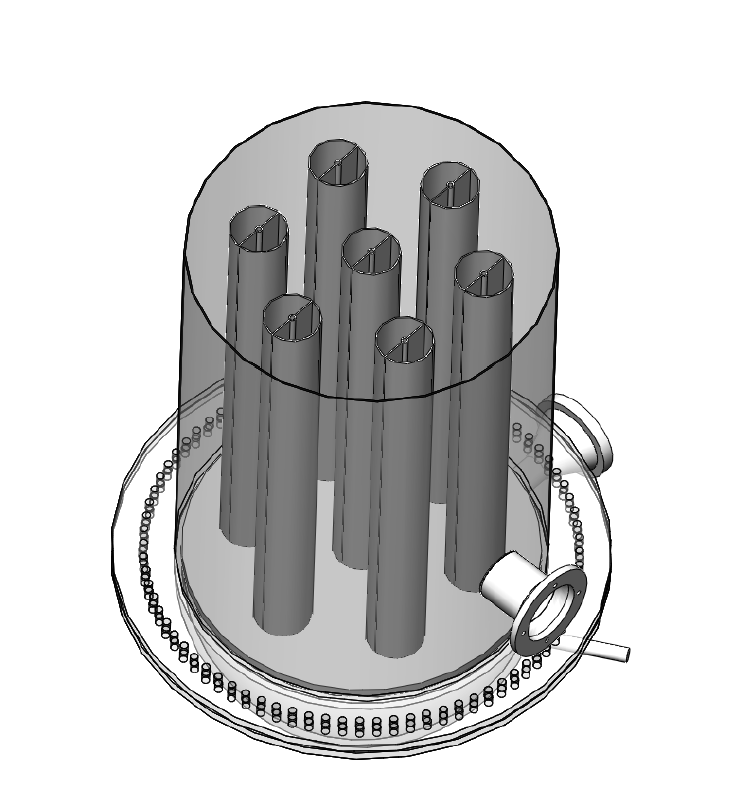
\includegraphics[width=\linewidth]{chapters/2-reaction/figures/FYD reactor 7 tubes cross section 3D.PNG}
    \caption{3D cross section of reactor tube arrangement}
    \label{fig:reactortubearrangement}
\end{wrapfigure}
The bundle of 7 tubes was arranged such that a clearance of \SI{230}{\milli \metre}, which exceeds the rule of thumb for minimum clearance of 0.25 times of tube diameter based on Primo et al \cite{primo_shell_2012} to maximise cooling heat transfer. 2 tube sheets were fitted at each ends of the shell to fix the tubes in position. A triangular tube arrangement was selected due to the more robust tube sheet construction \cite{primo_shell_2012}.  The arrangement of 7 tubes held by the tube sheet is shown in \cref{fig:reactortubearrangement}.


\subsubsection{Secondary cooling tube dimensions}
As mentioned in Section \ref{sec:tripleconctube}, the secondary cooling water system was implemented in a triple concentric tube (TCTHE) manner within the reactor tubes to prevent thermal runaway and hotspots. Each secondary cooling water tubes were designed to have a diameter of \SI{20}{\milli \metre} to achieve a flowrate $2.1 \times 10^{-4} m^3 s^{-1}$. The wall thickness was also set as \SI{5}{\milli \metre} for a standardised production. 
The arrangement of the secondary cooling tube within the reactor tubes can be visualised in the cross section figure \ref{fig:concentriccoolingwater}. 
\begin{figure}[H]
    \centering
    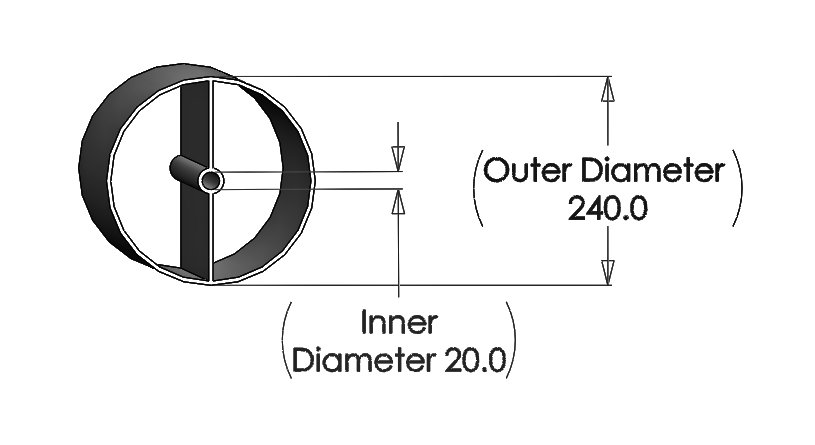
\includegraphics[width=0.65\linewidth]{chapters/2-reaction/figures/FYD conc tube with calc bw.png} 
    \caption{3D cross section of concentric secondary cooling water system}
    \label{fig:concentriccoolingwater}
\end{figure}

\subsubsection{Shell dimensions}
The diameter of the shell was 1.5m to withstand a total cooling water mass flowrate of \SI{2.3}{\kilogram \per \second}.
The minimum thickness of the shell ($e_{shell}$) was calculated using the equation \citeref{eqn:minthicknessshell},
\begin{equation}
    e_{shell} = \frac{p_dD_i}{2f-p_d} = \frac{0.11 \times 1500}{2 \times 143 - 0.11} = 0.577mm
    \label{eqn:minthicknessshell}
\end{equation}
where $D_i$ set as \SI{1500}{\milli \metre}, $p_d$ as 0.11 and $f$ value of 143$Nmm^{-2}$. The minimum thickness of the shell was calculated to be 0.577mm. After taking into account corrosion allowance of 1.5mm and other welding considerations, a final shell thickness of 5mm was chosen. 

\subsubsection{Head dimensions}
%A torispherical head was chosen as the preferred over ellipsoidal and hemispherical heads due to higher maximum stress and deformation threshold (). 
%Based on BS5500 (), the limitation of using torispherical head were checked and %\begin{equation}
    %\begin{split}
       % 0.02D \leq e \leq 0.12D \\
        %r \geq 0.06D \\
        %r \geq 2e \\
        %R \leq D
    %\end{split}
    %\label{eqn:torispherical}
%\end{equation}
The minimum thickness ($e_{head}$)of the hemispherical head was calculated using the equation \ref{eqn:hemisphericalend},
\begin{equation}
    e_{head} = \frac{pD_i}{4f-1.2p} = \frac{0.14 \times 1500}{4 \times 143 - 1.2 \times 0.14} = 0.26mm
    \label{eqn:hemisphericalend}
\end{equation}
with $p$ set as 1.4bar, $D_i$ set as 1500mm, $f$ value set as 143$Nmm^{-2}$.  The minimum thickness of the hemispherical end was calculated to be 0.26mm, but a final head thickness of 5mm was chosen to complement the thickness of the shell for ease of welding. 
%-refer BS5500 page 78 of the pdf

The minimum distance ($L_{im}$) between ports were calculated using the equation \ref{eqn:mindistance} below,
\begin{equation}
    L_m = \sqrt{(2r_{im}+e_{m})e_m} = \sqrt{(2 \times 1500 + 5)5} = 122.6mm
    \label{eqn:mindistance}
\end{equation}
where $r_{im}$ denotes the radius of inner diameter and $e_m$ denotes the thickness of the shell. The minimum distance between ports on the dome was calculated to be 122.6mm apart. 

%-label and explain this equation
%rewrite based on hemispherical
\subsection{Ports and flanges design}
A total of 7 ports were designed according to BS 5500:1997 and BS 1600:1991 standards. The 7 ports were namely:
%inlet and outlet ports for feed reactants, and one pressure relief valve (PRV). 
\begin{enumerate}
    \item Inlet of reactants
    \item Outlet of reactants
    \item Inlet of primary cooling water
    \item Outlet of primary cooling water
    \item Inlet of secondary cooling water
    \item Outlet of secondary cooling water
    \item Presure relief valve (PRV)
\end{enumerate}
Based on BS1600: 1991, schedule 40 pipes were chosen for all pipes \cite{noauthor_dimensions_nodate}. 
\subsubsection{Reactant flow port design}
The inlet and outlet of the reactant flow were placed at the top right and top left of the hemispherical shell domes respectively. Both ports were estimated to have an acceptable feed liquid velocity range (U) of 0.1 - 1 $ms^{-1}$. The cross sectional area (A) and pipe diameter (D) are then calculated using the volumetric flowrate ($Q_v$) as follows
\begin{align}
    A &= \frac{Q_v}{U} &
    \mathrm{D} &= \sqrt{\frac{4A}{\pi}}
\end{align}
where $Q_v$ is defined as $9.24 \times 10^{-4} m^3s^{-1}$ and a first approximation of $0.1 ms^{-1}$ liquid velocity was assumed to achieve a initial port diameter of 108.5mm. Based on BS 1600:1991, the diameter of the reactant inlet and outlet ports were chosen to have an OD of 114.3mm (4" NPS) with 6mm of wall thickness. 

\subsubsection{Cooling water flow port design}
Similarly, the outer diameter pipe diameter of both primary and secondary cooling water flow was calculated as previously described. The 
The diameter of the primary cooling water port was defined to have an OD of 219.1mm (8" NPS) with 6.55mm of wall thickness. The diameter of the secondary cooling tube were defined as OD of 60mm (2" NPS) with 4mm of wall thickness. All port dimensions were calculated based on information from BS 1600:1991. 


\subsubsection{Pressure relief valve design}
PRV was included as a safety device to protect the vessel and relief pressure in case of a overpressure event ().An overpressure event will occur when the pressure is beyond the design pressure (also known as maximum allowable working pressure, MAWP) \cite{marsha_lecture_nodate}. Detailed calculation based on API 250 standard \cite{api_standard_520_sizing_2013} of the sizing of safety relief valves for liquid can be viewed in Appendix section \ref{app:PRV}.

The PRV was designed to relief 20\% of the reactant flow within one minute. Due to highly flammable nature of nitration reaction, the maximum allowable accumulated pressure was designed for fire exposure at 1.21 ratio increase to the maximum allowable working pressure (MAWP), which is then calculated to be 1.74 bar. 

The final PRV size for schedule 40 steel was calculated to have an OD of 101.6mm (3 $\frac{1}{2}$" NPS) and a wall thickness of 5.74mm.
%- Inlet of water on top, outlet of water at the bottom. Size the water

%what is the arramgement of the piping? are we looking at all 19 stacked into one huge tube of diameter 100+cm? 


\subsubsection{Flange types and dimension}
Class 150 flanges was chosen from Table 16 of BS 1560:1989, based on the maximum permissible working pressure and temperature, which provides a suitable pressure-temperature rating for the stainless steel type 304L (material group 2.3). Weld-neck flanges was selected for all ports due to the high structural strength along with stress distribution \cite{ulma_forge_welding_2020}.
Based on JPI 75-48-73 standard, the nominal pipe size (NPS) for the flange was selected as 54" for class 150 flanges.
\subsubsection{Gasket type and dimension}
Gasket is a sealing material placed between flanges to create a leak-proof sealing \cite{varun_piping_nodate}. A narrow-faced, ring joint gasket type was chosen due to the suitability of design. The octagonal soft steel gasket was chosen to complement choice of ring joint gasket. The chosen gasket has a gasket factor (m) of 5.5 and minimum design seating stress (y) of 124 $Nmm^{-1}$. (BS5500)

\subsubsection{Bolt types and dimension}
The bolting material was selected was mild and carbon steel (BS 3692 grade 8.8), which is capable of withstanding 192 $N/mm^2$ design stress for temperature not exceeding 50C. Based on JPI 7S-48-73 standard for large diameter flanges, the diameter of bolt circle was defined as 1492mm, with 56 bolts of 32mm diameter each for 54" NPS flanges. 

\subsection{Overall design}
The overall cross section design of the reactor can be seen in \cref{fig:mainreactor} below. Additional mechanical design drawings from SolidWorks are included in \cref{app:engineeringdesign} .
\begin{figure}[h]
    \centering
    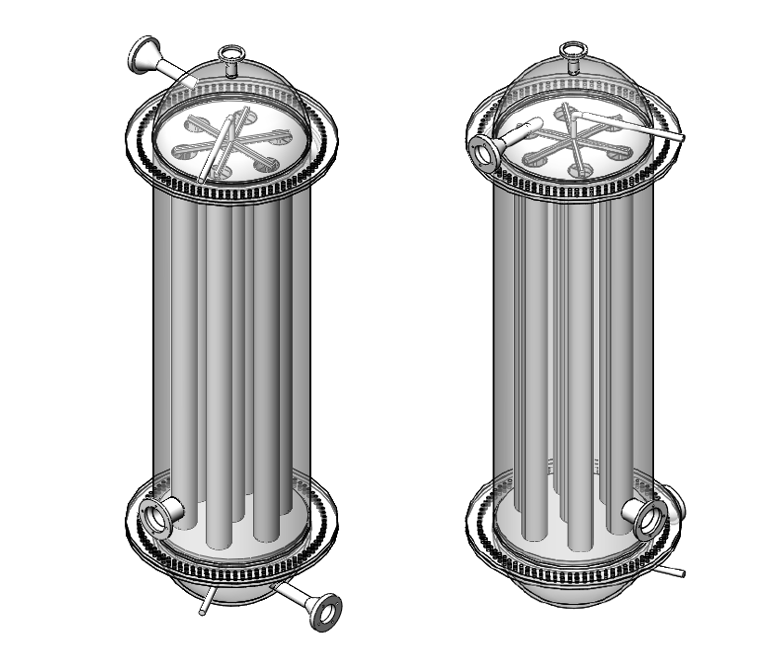
\includegraphics[width=0.6\linewidth]{chapters/2-reaction/figures/FYD reactor poster boy both.PNG}
    \caption{Overall design of reactor}
    \label{fig:mainreactor}
\end{figure}

